\documentclass{article}

\usepackage[utf8]{inputenc}
\usepackage{geometry}
\usepackage{listings}
\usepackage{graphicx}
\usepackage{geometry}
\usepackage{courier}

\graphicspath{{images/}}

\title{HW 3 \\ Integer Sort}
\author{Philip Nelson}
\date{2018 September 21}

\lstset{basicstyle=\footnotesize\ttfamily\normalsize,
        breaklines=true,
        stepnumber=1,
       }

\begin{document}

\maketitle

\section*{Introduction}

The purpose of this assignment is to write an MPI program that performs a parallel integer sort. It is written in the "master/slave" style. The process with id zero is the master; it generates an array of random integers. The master then sends chunks of the array to the slave processes to be sorted. When a slave receives a chunk, it sorts the data and returns it to the master. Once the master has sent out all the data, it waits to receive the sorted chunks from the slaves. As the sorted chunks are received, they are merged with the sorted array. Once all the chunks have been received and merged, the program reports the time that it took to sort the list and exits.

\section*{Code}

\begin{lstlisting}[showstringspaces=false, language=c++, numbers=left]
#include "random.hpp"
#include <algorithm>
#include <chrono>
#include <iostream>
#include <mpi.h>
#include <numeric>
#include <vector>

#define MCW MPI_COMM_WORLD

enum Tag
{
  UNSORTED,
  SORTED
};

std::vector<int> merge(std::vector<int> const& a, std::vector<int> const& b)
{
  std::vector<int> merged;
  unsigned int i = 0, j = 0;
  while (i < a.size() && j < b.size())
  {
    if (a[i] < b[j])
    {
      merged.push_back(a[i++]);
    }
    else
    {
      merged.push_back(b[j++]);
    }
  }

  std::copy(begin(a) + i, end(a), std::back_inserter(merged));
  std::copy(begin(b) + j, end(b), std::back_inserter(merged));

  return merged;
}

void random_fill(std::vector<int>::iterator b,
                 std::vector<int>::iterator e,
                 int low = 0,
                 int high = 1000)
{
  std::for_each(b, e, [&](int& a) { a = randInt(low, high); });
}

int main(int argc, char** argv)
{
  int rank, world_size;

  MPI_Init(NULL, NULL);
  MPI_Comm_rank(MCW, &rank);
  MPI_Comm_size(MCW, &world_size);

  if (0 == rank)
  {
    int n = 11;
    if (argc >= 2)
    {
      n = std::stoi(argv[1]);
    }

    /* ---------------------- */
    /* Generate Unsorted Data */
    /* ---------------------- */
    std::vector<int> unsorted;
    unsorted.resize(n);
    random_fill(std::begin(unsorted), std::end(unsorted));

    auto start = std::chrono::high_resolution_clock::now();
    /* ------------------------- */
    /* Send Unsorted Data Chunks */
    /* ------------------------- */
    const int chunksize = n / (world_size - 1);
    for (auto i = 0; i < world_size - 2; ++i)
    {
      MPI_Send((begin(unsorted) + (chunksize * i)).base(),
               chunksize,
               MPI_INT,
               i + 1,
               Tag::UNSORTED,
               MCW);
    }

    MPI_Send((begin(unsorted) + (chunksize * (world_size - 2))).base(),
             (chunksize + (n % chunksize)),
             MPI_INT,
             world_size - 1,
             Tag::UNSORTED,
             MCW);

    /* ------------------- */
    /* Receive Sorted Data */
    /* ------------------- */
    MPI_Status stat;
    std::vector<int> data;
    std::vector<int> result;
    int size;
    for (auto i = 0; i < world_size - 1; ++i)
    {
      MPI_Probe(MPI_ANY_SOURCE, Tag::SORTED, MCW, &stat);
      MPI_Get_count(&stat, MPI_INT, &size);
      data.resize(size);
      MPI_Recv(data.data(),
               size,
               MPI_INT,
               MPI_ANY_SOURCE,
               Tag::SORTED,
               MCW,
               MPI_STATUS_IGNORE);

      sorted = merge(sorted, data);
    }
    auto end = std::chrono::high_resolution_clock::now();
    auto total_time =
      std::chrono::duration<double, std::milli>(end - start).count();
    std::cout << "Time: " << total_time << " ms\n";
  }
  else
  {
    int n;
    MPI_Status stat;
    MPI_Probe(0, 0, MCW, &stat);
    MPI_Get_count(&stat, MPI_INT, &n);

    std::vector<int> data;
    data.resize(n);

    MPI_Recv(data.data(), n, MPI_INT, 0, Tag::UNSORTED, MCW, MPI_STATUS_IGNORE);
    std::sort(begin(data), end(data));
    MPI_Send(data.data(), n, MPI_INT, 0, Tag::SORTED, MCW);
  }

  MPI_Finalize();

  return EXIT_SUCCESS;
}
\end{lstlisting}

\section*{Output}

\begin{lstlisting}[showstringspaces=false]

# mpic++ main.cpp -O3 -o release.out

# mpiexec -n 4 release 100000

Time: 9.75266 ms

\end{lstlisting}

\section*{Findings}

I ran this program on lists of random integers from 100 to 1,000,000,000 elements and compared it's performance to std::sort running on a single thread. The results are detailed in Figure \ref{fig:graph}. The graph displays the ratio of MPI Sort to std::sort.
Lists upto 10,000 elements are sorted faster by std::sort but between 10,000 and 100,000,000 elements, the MIP Sort was faster. After 100,000,000 elements however, std::sort takes over as the faster sort.

My theory for this behavior is that sending the messages between threads becomes too expensive between 100,000,000 and 1,000,000,000 elements and std::sort is able to run faster with a single thread.


\begin{figure}[!htbp]
    \centering
    \fbox{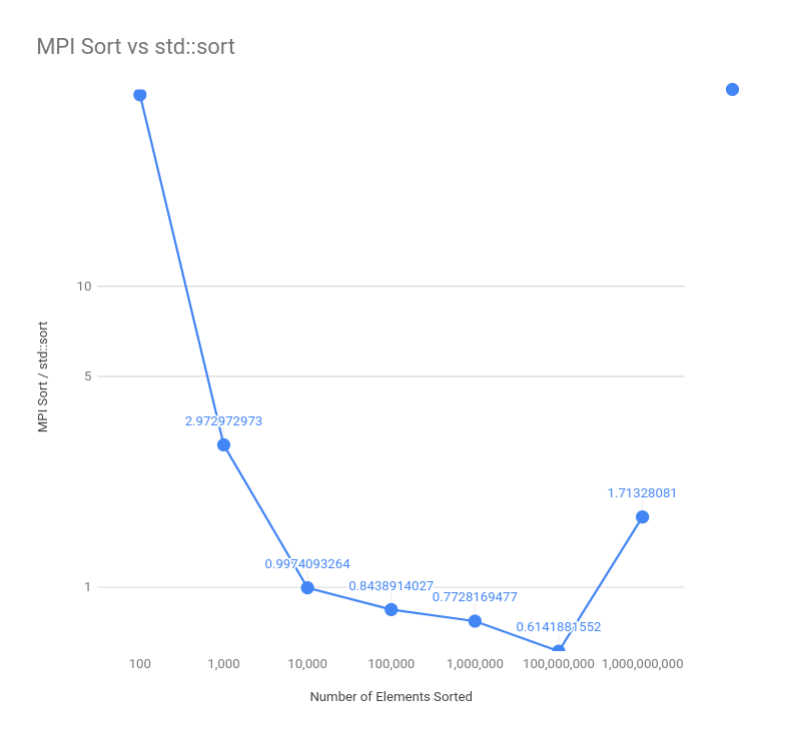
\includegraphics[width=150mm]{graph.png}}%tabe size
    \caption{MPI Sort vs std::sort}
    \label{fig:graph}
\end{figure}

\end{document}
